\documentclass{report}
\usepackage[utf8]{inputenc}
\usepackage[T1]{fontenc}
\usepackage[brazil]{babel}
\usepackage{graphicx}
\usepackage{amsfonts}
\usepackage{amssymb}
\usepackage{amsmath}
\usepackage{multicol}
\usepackage{ifthen}
\newboolean{firstanswerofthechapter}  
\usepackage{xcolor}
\colorlet{lightcyan}{cyan!40!white}
\usepackage{chngcntr}
\usepackage{stackengine}
\usepackage{tasks}
\usepackage{multirow}
\usepackage{float}
\newlength{\longestlabel}
\settowidth{\longestlabel}{\bfseries viii.}
%\settasks{counter-format={tsk[r].}, label-format={\bfseries}, label-width=\longestlabel,
    %item-indent=0pt, label-offset=2pt, column-sep={10pt}}
		
\setcounter{secnumdepth}{0} \setlength{\topmargin}{0cm}
\setlength{\headsep}{-0.3cm} \setlength{\textwidth}{17.5cm}
\setlength{\textheight}{23cm} \setlength{\oddsidemargin}{-0.8cm}
\setlength{\evensidemargin}{0cm} \setlength{\footskip}{-1.5cm}

		
\usepackage[lastexercise,answerdelayed]{exercise}
%\counterwithin{Exercise}{chapter}
%\counterwithin{Answer}{chapter}
%\renewcounter{Exercise}[chapter]
%\newcommand{\QuestionNB}{\bfseries\arabic{Question}.\ }
%\renewcommand{\ExerciseName}{Exercício}
%\renewcommand{\ExerciseHeader}{\noindent\def\stackalignment{l}% code from https://tex.stackexchange.com/a/195118/101651
    %\stackunder[0pt]{\colorbox{cyan}{\textcolor{white}{\textbf{\LARGE\ExerciseHeaderNB\;\large\ExerciseName}}}}{\textcolor{lightcyan}{\rule{\linewidth}{2pt}}}\medskip}
\renewcommand{\ExerciseName}{Exercícios}
\renewcommand{\ExerciseHeader}{\noindent\def\stackalignment{l}% code from https://tex.stackexchange.com/a/195118/101651
    \stackunder[0pt]{\colorbox{cyan}{\textcolor{white}{\textbf{\large\ExerciseName}}}}{\textcolor{lightcyan}{\rule{\linewidth}{2pt}}}\medskip}
%\renewcommand{\AnswerName}{Exercises}
%\renewcommand{\AnswerHeader}{\ifthenelse{\boolean{firstanswerofthechapter}}%
    %{\bigskip\noindent\textcolor{cyan}{\textbf{CHAPTER \thechapter}}\newline\newline%
        %\noindent\bfseries\emph{\textcolor{cyan}{\AnswerName\ \ExerciseHeaderNB, page %
                %\pageref{\AnswerRef}}}\smallskip}
    %{\noindent\bfseries\emph{\textcolor{cyan}{\AnswerName\ \ExerciseHeaderNB, page \pageref{\AnswerRef}}}\smallskip}}
%\setlength{\QuestionIndent}{16pt}

\begin{document}

\vspace*{-2cm}

\begin{center}
\begin{minipage}[s]{2cm}
\hspace{-1.3cm}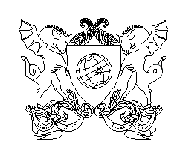
\includegraphics[scale=1.0]{/home/fsbmat/Documentos/GitHub/maf335.github.io/Brasao_UFV/brasaoufv.eps}
\end{minipage}
\begin{minipage}[s]{13cm}
{\begin{center} {\sc \Large Universidade Federal de Vi\c{c}osa}\\
{\sc \large Instituto de Ci\^encias Exatas e Tecnológicas}\\
{\sc \large Campus UFV - Florestal}\\
\end{center}}
\end{minipage}\begin{minipage}[s]{2 cm}
%\includegraphics[width=2 cm]{logoimecc.eps}
\end{minipage}
\end{center}

\vspace{-0.3cm}

%\hline \hline \noindent

%%%%%%%%%%%%%%%%%%%%%%%%%%%%%%%%%%%%%%%%%%%%%%%%%%%%%%%%%%%%%%%%%%%%%%%%%%%

\medskip

\begin{center}

\underline{\underline{{\large{\sc Lista de Álgebra Linear A - Lista 1}}}}

\bigskip

{\large {\bf Prof. Fernando Bastos}}
%\bigskip
%
%%{\sc Data: $19/06/2018$}
\end{center}


\begin{Exercise}

\begin{enumerate}

\item Sejam $A,B\in \mathbb{M}_{m\textrm{x}n}(\mathbb{K}).$ Mostre que:
\begin{tasks}
\task $(A+B)^{t}=A^{t}+B^{t}$
\task $(AB^{t})^{t}=BA^{t}$
\task Se $n=m,$ então $(AB)^{t}=B^{t}A^{t}$
\end{tasks} 

\item Sejam $A,B\in \mathbb{M}_{n}(\mathbb{K})$ e $\lambda\in \mathbb{R}.$ Mostre que:
\begin{tasks}
\task $det(AB)=detA.detB$
\task $det A=detA^{t}$
\task $det(\lambda A)=\lambda^{n}detA$
\end{tasks} 

\item Sejam $A,B\in \mathbb{M}_{n}(\mathbb{K})$ matrizes invertíveis. Mostre que:
\begin{tasks}
\task $det(A^{-1})=(detA)^{-1}$
\task $A^{-1}$ é invertível e $(A^{-1})^{-1}=A$
\task $AB$ é invertível e $(AB)^{-1}=B^{-1}A^{-1}$
\end{tasks} 






%%%%%%%%%%%%%%%%%%%%%%%%%%%%%%%%%%%%%%%%%%%%%%%%%%%%%%%%%%%%%%%%
%Exercicio 1
%%%%%%%%%%%%%%%%%%%%%%%%%%%%%%%%%%%%%%%%%%%%%%%%%%%%%%%%%%%%%%%%

\item \label{1lista1} Considere as matrizes $A, \ B, \ C, \ D
\textrm{ e } E$ com respectivas ordens, $4\times 3$, $4 \times 5$,
$3 \times 5$, $2 \times 5$ e $3 \times 5$. Determine quais das
seguintes expressões matriciais são possíveis e determine a
respectiva ordem.

$(a)$ $AE +B^T$; \hspace{1.4cm} $(b)$ $C(D^T +B)$;\hspace{1.4cm}
$(c)$ $AC+B$; \hspace{1.4cm} $(d)$ $E^T(CB)$.

%%%%%%%%%%%%%%%%%%%%%%%%%%%%%%%%%%%%%%%%%%%%%%%%%%%%%%%%%%%%%%%%
%Exercicio 2
%%%%%%%%%%%%%%%%%%%%%%%%%%%%%%%%%%%%%%%%%%%%%%%%%%%%%%%%%%%%%%%%

\item \label{1lista2} Determine as ordens das matrizes $A, \ B, \
C, \ D \textrm{ e } E$, sabendo que:

$AB^T$ tem ordem $5 \times 3$; \hspace{0.5cm} $(C^T+D)B$ tem ordem
$4 \times 6$ e \hspace{0.5cm} $E^TC$ tem ordem $5 \times 4$.

%%%%%%%%%%%%%%%%%%%%%%%%%%%%%%%%%%%%%%%%%%%%%%%%%%%%%%%%%%%%%%%%
%Exercicio 3
%%%%%%%%%%%%%%%%%%%%%%%%%%%%%%%%%%%%%%%%%%%%%%%%%%%%%%%%%%%%%%%%

\item \label{1lista3} Seja a matriz $A=\left[
\begin{array}{rrrrr}
1 & -3 & 7 & 8 & 2 \\
-4 & 0 & 11 & 3 & -6 \\
2 & -1 & 5 & 1& 3 \\
3 & 1 & -4 & 0 & 7
\end{array}
\right] $, determine :
\begin{enumerate}
 \item A ordem de $A$;
 \item Os elementos $a_{23}$, $a_{35}$ e $a_{43}$.
\end{enumerate}

%%%%%%%%%%%%%%%%%%%%%%%%%%%%%%%%%%%%%%%%%%%%%%%%%%%%%%%%%%%%%%%%
%Exercicio 4
%%%%%%%%%%%%%%%%%%%%%%%%%%%%%%%%%%%%%%%%%%%%%%%%%%%%%%%%%%%%%%%%

\item \label{1lista4} Sejam as matrizes $A, \ B, \ C, \ D \textrm{
e } E$ que verificam $ABCDE = EDCBA$, sabendo que $C$ é uma matriz
de ordem $3 \times 2$, quais são as ordens das outras quatro
matrizes?

%%%%%%%%%%%%%%%%%%%%%%%%%%%%%%%%%%%%%%%%%%%%%%%%%%%%%%%%%%%%%%%%
%Exercicio 5
%%%%%%%%%%%%%%%%%%%%%%%%%%%%%%%%%%%%%%%%%%%%%%%%%%%%%%%%%%%%%%%%

\item \label{1lista5} Sejam as matrizes $A=\left[
\begin{array}{rrrr}
1 & -1 & 3 & 2 \\
0 &  1 & 4 & -3 \\
1 & 2 & -1 & 5
\end{array}
\right] $,  $B=\left[
\begin{array}{rrr}
0 & 3 &  2 \\
-2 & 1 & 4 \\
-1 & 2 & 1 \\
4 & 3 & 1
\end{array}
\right],$ $C = A\cdot B$ e $D=B \cdot A$. Determine os elementos
$c_{32}$ e $d_{43}$.


%%%%%%%%%%%%%%%%%%%%%%%%%%%%%%%%%%%%%%%%%%%%%%%%%%%%%%%%%%%%%%%%
%Exercicio 6
%%%%%%%%%%%%%%%%%%%%%%%%%%%%%%%%%%%%%%%%%%%%%%%%%%%%%%%%%%%%%%%%

\item \label{1lista6} Determine a matriz quadrada, $A=(a_{ij})$,
de ordem $4$ cujos elementos são dados por: 
$$
a_{ij}= \left\{
\begin{array}{rr}
2i-3j, & \textrm{ se }  \ i<j \\
i^2+2j, & \textrm{ se } \ i=j \\
-3i+4j, & \textrm{ se } \ i>j
\end{array}\right.
$$

%%%%%%%%%%%%%%%%%%%%%%%%%%%%%%%%%%%%%%%%%%%%%%%%%%%%%%%%%%%%%%%%
%Exercicio 7
%%%%%%%%%%%%%%%%%%%%%%%%%%%%%%%%%%%%%%%%%%%%%%%%%%%%%%%%%%%%%%%%

\item \label{1lista7} Seja a matriz $A=\left[
\begin{array}{rr}
2 & -1 \\
3 & -2
\end{array}
\right]$, determine:

$(a)$ $A^2$; \hspace{1.5cm} $(b)$ $A^3$;\hspace{1.5cm} $(c)$
$A^{31}$; \hspace{1.5cm} $(d)$ $A^{42}$.

%%%%%%%%%%%%%%%%%%%%%%%%%%%%%%%%%%%%%%%%%%%%%%%%%%%%%%%%%%%%%%%%
%Exercicio 8
%%%%%%%%%%%%%%%%%%%%%%%%%%%%%%%%%%%%%%%%%%%%%%%%%%%%%%%%%%%%%%%%

\item \label{1lista8} Determine números reais $x$ e $y$ tais que
$$\left[
\begin{array}{rr}
x^3 & y^2 \\
y^2 & x^2
\end{array}
\right] +  \left[
\begin{array}{rr}
-x & 3y \\
4y & 2x
\end{array}
\right] =  \left[
\begin{array}{rr}
0 & 4 \\
5 & -1
\end{array}
\right].$$

%%%%%%%%%%%%%%%%%%%%%%%%%%%%%%%%%%%%%%%%%%%%%%%%%%%%%%%%%%%%%%%%
%Exercicio 9
%%%%%%%%%%%%%%%%%%%%%%%%%%%%%%%%%%%%%%%%%%%%%%%%%%%%%%%%%%%%%%%%

\item \label{1lista9} Determine, em cada um dos casos abaixo, $x$,
$y$ e $z$ números reais tais que a matriz $A$ seja simétrica.

$(a)$ $A=\left[
\begin{array}{cc}
-2 & x \\
4 & 1
\end{array}
\right] $, \hspace{0.5cm}  $(b)$ $A=\left[
\begin{array}{ccc}
8 & x+3 & -10 \\
15 &  -5 & -8 \\
y-2 & 2z & 9
\end{array}
\right] $,  \hspace{0.5cm} $(c)$ $A=\left[
\begin{array}{ccc}
8 & x^2+3 &  -5 \\
7 & -9 & 4 \\
y+x & z+3x & 11
\end{array}
\right].$

%%%%%%%%%%%%%%%%%%%%%%%%%%%%%%%%%%%%%%%%%%%%%%%%%%%%%%%%%%%%%%%%
%Exercicio 10
%%%%%%%%%%%%%%%%%%%%%%%%%%%%%%%%%%%%%%%%%%%%%%%%%%%%%%%%%%%%%%%%

\item \label{1lista10} Considere as matrizes:

$ A=\left[
\begin{array}{rr}
3 & 0 \\
-1 & 2 \\
1 & 1
\end{array}
\right]$,   $B=\left[
\begin{array}{rr}
4 & -1 \\
0 & 2
\end{array}
\right]$,  $C=\left[
\begin{array}{ccc}
1 & 4 & 2 \\
3 & 1 & 5
\end{array}
\right]$,  $D=\left[
\begin{array}{rrr}
1 & 5 & 2 \\
-1 & 0 & 1 \\
3 & 2 & 4
\end{array}
\right]$,  $E=\left[
\begin{array}{rrr}
6 & 1 & 3 \\
-1 & 1 & 2 \\
4 & 1 & 3
\end{array}
\right]$.

Quando possível, calcule o que se pede.

$(a)$ $4E-2D$; \hspace{1cm} $(b)$ $2A^{T}+C$; \hspace{1cm} $(c)$
$\left( 2E^{T}-3D^{T}\right) ^{T}$; \hspace{1cm} $(d)$ $\left(
BA^{T}-2C\right) ^{T}$;

$(e)$ $\left( -AC\right) ^{T}+5D^{T}$; \hspace{1cm} $(f)$
$B^{T}\left( CC^{T}-A^{T}A\right) $; \hspace{1cm} $(g)$
$D^{T}E^{T}-\left( ED\right) ^{T}$.

%%%%%%%%%%%%%%%%%%%%%%%%%%%%%%%%%%%%%%%%%%%%%%%%%%%%%%%%%%%%%%%%
%Exercicio 11
%%%%%%%%%%%%%%%%%%%%%%%%%%%%%%%%%%%%%%%%%%%%%%%%%%%%%%%%%%%%%%%%

\item \label{1lista11} Diz-se que uma matriz $B$ é uma {\it raiz
quadrada de} (uma matriz) $A$ se $B^{2}=A$.

\begin{enumerate}
\item  Encontre duas raízes quadradas de $A=\left[
\begin{array}{cc}
2 & 2 \\
2 & 2
\end{array}
\right] $.

\item  Existem quantas raízes quadradas distintas de $A=\left[
\begin{array}{cc}
5 & 0 \\
0 & 9
\end{array}
\right] $? Justifique.

\item  Na sua opinião qualquer matriz $2\times 2$ tem pelo menos
uma raiz quadrada? Explique seu raciocínio.
\end{enumerate}

%%%%%%%%%%%%%%%%%%%%%%%%%%%%%%%%%%%%%%%%%%%%%%%%%%%%%%%%%%%%%%%%
%Exercicio 12
%%%%%%%%%%%%%%%%%%%%%%%%%%%%%%%%%%%%%%%%%%%%%%%%%%%%%%%%%%%%%%%%

\item \label{1lista12} Sejam $A$ e $B$ matrizes em $M_n(\real)$,
se $AB=BA$, mostre que:

$(a)$ $(A\pm B)^2 = A^2 \pm 2AB+B^2$, \hspace{2cm} $(b)$
$(A-B)(A+B) = A^2 - B^2$,

$(c)$ $(A-B)(A^2 +AB+B^2) = A^3 - B^3$.

%%%%%%%%%%%%%%%%%%%%%%%%%%%%%%%%%%%%%%%%%%%%%%%%%%%%%%%%%%%%%%%%
%Exercicio 13
%%%%%%%%%%%%%%%%%%%%%%%%%%%%%%%%%%%%%%%%%%%%%%%%%%%%%%%%%%%%%%%%

\item \label{1lista13} Seja $A$ matriz em $M_n(\real)$, mostre
que:

$(a)$ As matrizes $A\cdot A^T$ e $\frac{1}{2}(A+A^T)^2$ são
simétricas,

$(b)$ A matriz $\frac{1}{2}(A-A^T)^2$ é anti-simétrica,

$(c)$ Toda matriz quadrada é a soma de uma matriz simétrica com
uma matriz anti-simétrica.

%%%%%%%%%%%%%%%%%%%%%%%%%%%%%%%%%%%%%%%%%%%%%%%%%%%%%%%%%%%%%%%%
%Exercicio 14
%%%%%%%%%%%%%%%%%%%%%%%%%%%%%%%%%%%%%%%%%%%%%%%%%%%%%%%%%%%%%%%%

\item \label{1lista14} Dizemos que uma matriz quadrada $A$ é
ortogonal se, e somente se, $A\cdot A^T = I$. Determine:

$(a)$ Os possíveis valores para o determinante de uma matriz
ortogonal.

$(b)$ Quantas matrizes reais de ordem $2$ são simultaneamente
anti-simétricas e ortogonais.

%%%%%%%%%%%%%%%%%%%%%%%%%%%%%%%%%%%%%%%%%%%%%%%%%%%%%%%%%%%%%%%%
%Exercicio 15
%%%%%%%%%%%%%%%%%%%%%%%%%%%%%%%%%%%%%%%%%%%%%%%%%%%%%%%%%%%%%%%%

\item \label{1lista15} Determine o número real $m$ de modo que a
matriz $ M=\left[
\begin{array}{rr}
-1 & 0 \\
0 & m
\end{array}
\right]$ seja ortogonal.

%%%%%%%%%%%%%%%%%%%%%%%%%%%%%%%%%%%%%%%%%%%%%%%%%%%%%%%%%%%%%%%%
%Exercicio 16
%%%%%%%%%%%%%%%%%%%%%%%%%%%%%%%%%%%%%%%%%%%%%%%%%%%%%%%%%%%%%%%%

\item \label{1lista16} Verifique quais das matrizes abaixo é
ortogonal.

$ A=\left[
\begin{array}{rr}
0 & 1 \\
1 & 0
\end{array}
\right]$,  \hspace{0.7cm} $B=\left[
\begin{array}{rr}
1 & -2 \\
2 & 1
\end{array}
\right]$, \hspace{0.7cm} $C=\left[
\begin{array}{cc}
\frac{1}{3} & \frac{2\sqrt{2}}{3} \\
&  \\
\frac{2\sqrt{2}}{3} & -\frac{1}{3}
\end{array}
\right]$, \hspace{0.7cm} $D=\left[
\begin{array}{rrr}
\frac{\sqrt{3}}{3} & \frac{\sqrt{3}}{3} & \frac{\sqrt{3}}{3} \\
& & \\
-\frac{\sqrt{6}}{3} & \frac{\sqrt{6}}{6} & \frac{\sqrt{6}}{6} \\
& & \\
0 & -\frac{\sqrt{2}}{2} & \frac{\sqrt{2}}{2}
\end{array}
\right]$.

%%%%%%%%%%%%%%%%%%%%%%%%%%%%%%%%%%%%%%%%%%%%%%%%%%%%%%%%%%%%%%%%
%Exercicio 17
%%%%%%%%%%%%%%%%%%%%%%%%%%%%%%%%%%%%%%%%%%%%%%%%%%%%%%%%%%%%%%%%

\item \label{1lista17} Dado $\alpha$ número real considere a
matriz $T_\alpha=\left[
\begin{array}{rr}
\cos \alpha & -\sin \alpha \\
\sin \alpha & \cos \alpha
\end{array}
\right]$.

$(a)$ Dados $\alpha$ e $\beta$ em $\real$, mostre que $T_\alpha
\cdot T_\beta = T_{\alpha +\beta}$.

$(b)$ Calcule $T_{-\alpha}$.

$(c)$ Mostre que para todo número $\alpha$ a matriz $T_\alpha$ é
ortogonal.


%%%%%%%%%%%%%%%%%%%%%%%%%%%%%%%%%%%%%%%%%%%%%%%%%%%%%%%%%%%%%%%%
%Exercicio 18
%%%%%%%%%%%%%%%%%%%%%%%%%%%%%%%%%%%%%%%%%%%%%%%%%%%%%%%%%%%%%%%%

\item \label{1lista18}  Seja $A=\left[
\begin{array}{cccc}
  a_{11} & a_{12} & \cdots & a_{1n} \\
  a_{21} & a_{22} & \cdots & a_{2n} \\
  & \cdots & \cdots & \\
  a_{n1} & a_{n2} & \cdots & a_{nn} \\
\end{array}
\right],$ uma matriz quadrada de ordem $n$. O {\it traço de} $A$,
denotado por $tr \ (A)$, é definido como sendo o número real: $$
tr \ (A) = \sum_{k=1}^{n}a_{kk} = a_{11} + a_{22} + \cdots
a_{nn},$$
 ou seja, o traço de $A$ é a soma dos elementos da diagonal
 principal de $A$.

Dadas $A$ e $B$ matrizes quadradas de ordem $n$, valem as
seguintes propriedades:

$(a)$  $tr \ ( A+B) = tr \ ( A) + tr \ ( B) $; \hspace{1cm} $(b)$
$tr \ (kA)  =k \ tr \ (A) $, onde $k \in \real$;

$(c)$ $tr \ (A^T) =tr \ (A) $; \hspace{3.3cm} $(d)$ $tr \ (AB) =tr
\ (BA)$.

Usando algumas destas propriedades verifique que não existem $A$ e
$B$ matrizes quadradas de ordem $n$ tais que $AB-BA=I$.

%%%%%%%%%%%%%%%%%%%%%%%%%%%%%%%%%%%%%%%%%%%%%%%%%%%%%%%%%%%%%%%%

%%%%%%%%%%%%%%%%%%%%%%%%%%%%%%%%%%%%%%%%%%%%%%%%%%%%%%%%%%%%%%%%
%Exercicio 19
%%%%%%%%%%%%%%%%%%%%%%%%%%%%%%%%%%%%%%%%%%%%%%%%%%%%%%%%%%%%%%%%

\item \label{1lista19} Verifique que se $A$ é uma matriz $m\times
n$, então os traços de $AA^{T}$ e $A^{T}A$ estão definidos. Em
seguida, prove que $tr \ (AA^{T}) =tr \ ( A^{T}A)$.


%%%%%%%%%%%%%%%%%%%%%%%%%%%%%%%%%%%%%%%%%%%%%%%%%%%%%%%%%%%%%%%%
%Exercicio 20
%%%%%%%%%%%%%%%%%%%%%%%%%%%%%%%%%%%%%%%%%%%%%%%%%%%%%%%%%%%%%%%%

\item \label{1lista20} Mostre que se $A^{T}A=A$, então $A$ é
simétrica e $A=A^{2}$.


%%%%%%%%%%%%%%%%%%%%%%%%%%%%%%%%%%%%%%%%%%%%%%%%%%%%%%%%%%%%%%%%
%Exercicio 21
%%%%%%%%%%%%%%%%%%%%%%%%%%%%%%%%%%%%%%%%%%%%%%%%%%%%%%%%%%%%%%%%

\item \label{1lista21} Suponha que $A$ é uma matriz quadrada e que
$D$ é uma matriz diagonal tal que $AD=I$. O que se pode afirmar
sobre a matriz $A$? Explique seu raciocínio.


%%%%%%%%%%%%%%%%%%%%%%%%%%%%%%%%%%%%%%%%%%%%%%%%%%%%%%%%%%%%%%%%
%Exercicio 22
%%%%%%%%%%%%%%%%%%%%%%%%%%%%%%%%%%%%%%%%%%%%%%%%%%%%%%%%%%%%%%%%

%\item \label{1lista22}  Encontre uma matriz triangular superior
%tal que $ A^{3}=\left[
%\begin{array}{cc}
%1 & 30 \\
%0 & -8
%\end{array}
%\right].
%$

%%%%%%%%%%%%%%%%%%%%%%%%%%%%%%%%%%%%%%%%%%%%%%%%%%%%%%%%%%%%%%%%
%Exercicio 22
%%%%%%%%%%%%%%%%%%%%%%%%%%%%%%%%%%%%%%%%%%%%%%%%%%%%%%%%%%%%%%%%

\item \label{1lista22}  Considere a matriz $A=\left[
\begin{array}{cccc}
a_{11} & 0 & \cdots  & 0 \\
0 & a_{22} & \cdots  & 0 \\
\vdots  & \vdots  & \ddots  & \vdots  \\
0 & 0 & \cdots  & a_{nn}
\end{array}
\right],$ onde $a_{11}a_{22}...a_{nn}\neq 0$. Determine $A^{-1}$,
a inversa de $A$, se existir.

%%%%%%%%%%%%%%%%%%%%%%%%%%%%%%%%%%%%%%%%%%%%%%%%%%%%%%%%%%%%%%%%

%\item Considere a matriz
%$$
%A=\left[
%\begin{array}{cc}
%a & b \\
%c & d
%\end{array}
%\right],$$ onde $ab-cd\neq 0$. Prove que $A$ é invertível. (Dica:
%use sua intuição para inferir um candidato à inversa de $A$).


%%%%%%%%%%%%%%%%%%%%%%%%%%%%%%%%%%%%%%%%%%%%%%%%%%%%%%%%%%%%%%%%
%\item Use o exercício \ref{1lista19} para encontrar a inversa de
%$$
%\left[
%\begin{array}{rr}
%\cos \theta  & \func{sen}\theta  \\
%-\func{sen}\theta  & \cos \theta
%\end{array}
%\right].$$

%%%%%%%%%%%%%%%%%%%%%%%%%%%%%%%%%%%%%%%%%%%%%%%%%%%%%%%%%%%%%%%%
%Exercicio 23
%%%%%%%%%%%%%%%%%%%%%%%%%%%%%%%%%%%%%%%%%%%%%%%%%%%%%%%%%%%%%%%%

\item \label{1lista23} Prove que se $A$ é inversível e $AB=AC$,
então $B=C$.


%%%%%%%%%%%%%%%%%%%%%%%%%%%%%%%%%%%%%%%%%%%%%%%%%%%%%%%%%%%%%%%%
%Exercicio 24
%%%%%%%%%%%%%%%%%%%%%%%%%%%%%%%%%%%%%%%%%%%%%%%%%%%%%%%%%%%%%%%%

\item \label{1lista24} É possível ter $AB=I$ e $B$ não ser a
inversa de A? Justifique sua resposta!



%%%%%%%%%%%%%%%%%%%%%%%%%%%%%%%%%%%%%%%%%%%%%%%%%%%%%%%%%%%%%%%%
%Exercicio 25
%%%%%%%%%%%%%%%%%%%%%%%%%%%%%%%%%%%%%%%%%%%%%%%%%%%%%%%%%%%%%%%%

\item \label{1lista25}  Seja $A$ uma matriz quadrada de ordem $n$,
mostre que:
\begin{enumerate}
    \item Se $A$ satisfaz a igualdade $ A^{2}-3A+I=0$, então
    $A^{-1}=3I-A$.
    \item Se $A$ é tal que $A^{n+1}=0$, então
    $(I-A)^{-1}=I+A+A^{2}+...+A^{n}.$
\end{enumerate}


%%%%%%%%%%%%%%%%%%%%%%%%%%%%%%%%%%%%%%%%%%%%%%%%%%%%%%%%%%%%%%%%
%Exercicio 26
%%%%%%%%%%%%%%%%%%%%%%%%%%%%%%%%%%%%%%%%%%%%%%%%%%%%%%%%%%%%%%%%

\item \label{1lista26} Decida se a afirmação dada é (sempre)
verdadeira ou (às vezes) falsa. Justifique sua resposta dando um
argumento lógico matemático ou um contra-exemplo.

\begin{enumerate}
\item  (\quad ) Se a primeira coluna de $A$ for constituída
somente de zeros, o mesmo ocorre com a primeira coluna de qualquer
produto $AB$.

\item  (\quad ) Se a primeira linha de $A$ for constituída somente
de zeros, o mesmo ocorre com a primeira linha de qualquer produto
$AB$.

\item  (\quad ) Se a soma de matrizes $AB+BA$ estiver definida,
então $A$ e $B$ devem ser matrizes quadradas.

\item  (\quad ) Se $A$ é uma matriz quadrada com duas linhas
idênticas, então $A^{2}$ tem duas linhas idênticas.

\item  (\quad ) Se $A$ é uma matriz quadrada e $A^{2}$ tem uma
coluna constituída somente de zeros, então necessariamente $A$ tem
uma coluna constituída somente de zeros.

\item  (\quad ) Se $AA^{T}$ é uma matriz singular, então $A$ não é
invertível.

\item  (\quad ) Se $A$ é invertível e $AB=0$, então
necessariamente $B$ é a matriz nula.

\item  (\quad ) A soma de duas matrizes inversíveis é sempre uma
matriz invertível (não singular).

\item  (\quad ) Se $A$ é uma matriz quadrada tal que $A^{4}=0$,
então
$$
(I-A)^{-1}=I+A+A^{2}+A^{3}.
$$
\end{enumerate}





%Supondo que $A$ e $B$ são matrizes quadradas de ordem $n$
%inversíveis, prove as seguintes igualdades:

%\begin{enumerate}
%\item $(A^{-1} + B^{-1})^{-1} = A (A + B)^{-1} B.$

%\item $(I +AB)^{-1} A = A (I + BA)^{-1}$.

%\item $(A + BB^T)B = A^{-1} B (I +B^TA^{_1}B)^{-1}.$

%\end{enumerate}

%%%%%%%%%%%%%%%%%%%%%%%%%%%%%%%%%%%%%%%%%%%%%%%%%%%%%%%%%%%%%%%

%%%%%%%%%%%%%%%%%%%%%%%%%%%%%%%%%%%%%%%%%%%%%%%%%%%%%%%%%%%%%%%%
%Exercicio 27
%%%%%%%%%%%%%%%%%%%%%%%%%%%%%%%%%%%%%%%%%%%%%%%%%%%%%%%%%%%%%%%%

\item \label{1lista27} Seja $A$ uma matriz quadrada de ordem $5$,
cujo determinante é igual a $-3$, pede-se:
\begin{enumerate}
    \item O determinante da matriz $P$ dada por $P=4A^{-1}A^T$.
    \item Dedicir se $P$ é ou não inversível.
    \item O determinante da matriz $B$ obtida de $A$ após serem
    realizadas as seguintes operações: $L_3\leftrightarrow L_2$;
    $L_1 \rightarrow L_1 + 2L_5$; $L_4 \rightarrow -3 L_4$.
    \item Dedicir se a matriz $Q=AA^T$ é ou não inversível.
\end{enumerate}


%%%%%%%%%%%%%%%%%%%%%%%%%%%%%%%%%%%%%%%%%%%%%%%%%%%%%%%%%%%%%%%%
%Exercicio 28
%%%%%%%%%%%%%%%%%%%%%%%%%%%%%%%%%%%%%%%%%%%%%%%%%%%%%%%%%%%%%%%%

\item \label{1lista28} Calcule o determinante da matriz $A= \left[
\begin{array}{rrrr}
4 & -5 & 3 & 2 \\
-1 & 0 & 3 & 0 \\
1 & 2 & -1 & 3 \\
2 & 1 & 0 & 4
\end{array}
\right];$
\begin{enumerate}
    \item Desenvolvendo-o pela segunda linha (usando cofatores)
    \item Pelo processo de triangulação (usando operações
    elementares sobre as linhas da matriz.
\end{enumerate}

%%%%%%%%%%%%%%%%%%%%%%%%%%%%%%%%%%%%%%%%%%%%%%%%%%%%%%%%%%%%%%%%
%Exercicio 29
%%%%%%%%%%%%%%%%%%%%%%%%%%%%%%%%%%%%%%%%%%%%%%%%%%%%%%%%%%%%%%%%

\item \label{1lista29} Dadas as matrizes $A= \left[
\begin{array}{rrrr}
1 & -5 & -1 & 2 \\
0 & 2 & -3 & 4 \\
0 & 0 & 4 & -2 \\
0 & 0 & 0 & 3
\end{array}
\right]$ e $B= \left[
\begin{array}{rrrr}
-3 & 0 & 0 & 0 \\
3 & -4 & 0 & 0 \\
2 & 2 & -1 & 0 \\
2 & 1 & 1 & -2
\end{array}
\right],$ determine:

$(a)$ $\det (AB)$; \hspace{0.5cm} $(b)$ $A^{-1}$; \hspace{0.5cm}
$(c)$ $B^{-1}$; \hspace{0.5cm} $(d)$ $(AB)^{-1}$; \hspace{0.5cm}
$(e)$ $\det C$, onde $C A^T=2BC^2$.

%%%%%%%%%%%%%%%%%%%%%%%%%%%%%%%%%%%%%%%%%%%%%%%%%%%%%%%%%%%%%%%%
%Exercicio 30
%%%%%%%%%%%%%%%%%%%%%%%%%%%%%%%%%%%%%%%%%%%%%%%%%%%%%%%%%%%%%%%%

\item \label{1lista30} Seja $Q$ uma matriz quadrada de ordem $n$
tal que $\det Q \ne 0$ e $Q^3 +2 Q^2 =0$, determine o valor de
$\det Q$.


%%%%%%%%%%%%%%%%%%%%%%%%%%%%%%%%%%%%%%%%%%%%%%%%%%%%%%%%%%%%%%%%
%Exercicio 31
%%%%%%%%%%%%%%%%%%%%%%%%%%%%%%%%%%%%%%%%%%%%%%%%%%%%%%%%%%%%%%%%

\item \label{1lista31} Dada a matriz $A= \left[
\begin{array}{rrrr}
1 & 5 & -1 & 3 \\
-1 & 2 & -2 & 4 \\
6 & 7 & 3 & -1 \\
5 & 3 & 0 & 4
\end{array}
\right]$, determine:

$(a)$ $\det A$ utilizando as operações elementares sobre as linhas
de $A$;

$(b)$ $\det A^T$; \hspace{0.5cm} $(c)$ $\det A^2$; \hspace{0.5cm}
$(d)$ $A^{-1}$; \hspace{0.5cm} $(e)$ $\det -A$; \hspace{0.5cm}
$(f)$ $3AA^T$.

%%%%%%%%%%%%%%%%%%%%%%%%%%%%%%%%%%%%%%%%%%%%%%%%%%%%%%%%%%%%%%%%
%Exercicio 32
%%%%%%%%%%%%%%%%%%%%%%%%%%%%%%%%%%%%%%%%%%%%%%%%%%%%%%%%%%%%%%%%

\item \label{1lista32} Seja a matriz $A=\left[
\begin{array}{rrr}
1 & 1 & -1 \\
1 & 0 & 1 \\
0 & 1 & 1
\end{array}
\right].$
\begin{enumerate}
    \item Determine o polinômio $p(x)=\det (xI_3 -A)$, onde $I_3$
    é a matriz identidade de ordem $3$ e $x \in \real$.
    \item Verifique que $p(A)=0$, onde $0$ é a matriz nula $3
    \times 3$.
    \item Use o item $(b)$ para calcular a inversa de $A$.
\end{enumerate}

%%%%%%%%%%%%%%%%%%%%%%%%%%%%%%%%%%%%%%%%%%%%%%%%%%%%%%%%%%%%%%%%
%Exercicio 33
%%%%%%%%%%%%%%%%%%%%%%%%%%%%%%%%%%%%%%%%%%%%%%%%%%%%%%%%%%%%%%%%

\item \label{1lista33}  Calcule os seguintes determinantes:

\medskip

$(a)$   $\left|
\begin{array}{rrr}
2 & -1 & 5 \\
1 & 9 & -4 \\
3 & 0 & 0
\end{array}
\right|; $ \hspace{2cm} $(b)$ $\left|
\begin{array}{ccc}
1+a & b & c \\
a & 1+b & c \\
a & b & 1+c
\end{array}
\right|;$   \hspace{1.1cm} $(c)$ $\left|
\begin{array}{ccc}
c & -4 & 3 \\
2 & 1 & c^{2} \\
4 & c-1 & 2
\end{array}
\right|; $

\bigskip

$(d)$  $\left|
\begin{array}{rrrr}
4 & -5 & 3 & 2 \\
-1 & 0 & 3 & 0 \\
1 & 2 & -1 & 3 \\
2 & 1 & 0 & 4
\end{array}
\right|;$ \hspace{1cm} $(e)$ $\left|
\begin{array}{rrrrr}
0 & 0 & 0 & 0 & -3 \\
0 & 0 & 0 & -4 & 0 \\
0 & 0 & -1 & 0 & 0 \\
0 & 2 & 0 & 0 & 0 \\
5 & 0 & 0 & 1 & 0
\end{array}
\right|;$ \hspace{1cm} $(f)$ $\left|
\begin{array}{rrrrr}
5 & 0 & 0 & 0 & 0 \\
0 & 0 & 0 & 0 & -4 \\
0 & 0 & 3 & 0 & 0 \\
0 & 0 & 0 & 1 & 0 \\
0 & -2 & 0 & 0 & 0
\end{array}
\right|.$


%%%%%%%%%%%%%%%%%%%%%%%%%%%%%%%%%%%%%%%%%%%%%%%%%%%%%%%%%%%%%%%%
%Exercicio 34
%%%%%%%%%%%%%%%%%%%%%%%%%%%%%%%%%%%%%%%%%%%%%%%%%%%%%%%%%%%%%%%%

\item \label{1lista34} Resolva as seguintes equações:

$(a)$ $ \left|
\begin{array}{ccc}
x & 5 & 7 \\
0 & x+1 & 6 \\
0 & 0 & 2x-1
\end{array}
\right| =0;$ \ $(b)$ $ \left|
\begin{array}{ccc}
2 & x-2 & 3 \\
2x+3 & x-1 & 4 \\
5 & 1 & 0
\end{array}
\right| =16;$ \ $(c)$ $ \left|
\begin{array}{cc}
x & -1 \\
3 & 1-x
\end{array}
\right| =\left|
\begin{array}{ccc}
1 & 0 & -3 \\
2 & x & -6 \\
1 & 3 & x-5
\end{array}
\right|.$

%%%%%%%%%%%%%%%%%%%%%%%%%%%%%%%%%%%%%%%%%%%%%%%%%%%%%%%%%%%%%%%%
%Exercicio 22
%%%%%%%%%%%%%%%%%%%%%%%%%%%%%%%%%%%%%%%%%%%%%%%%%%%%%%%%%%%%%%%%

%\item \label{1lista22}  Seja $A=\left[
%\begin{array}{rrr}
%-2 & 2 & 3 \\
%-2 & 3 & 2 \\
%-4 & 2 & 5
%\end{array}
%\right] $. Determine $x$, número real,  tal que $\det ( xI-A) =0$.



%%%%%%%%%%%%%%%%%%%%%%%%%%%%%%%%%%%%%%%%%%%%%%%%%%%%%%%%%%%%%%%%
%Exercicio 35
%%%%%%%%%%%%%%%%%%%%%%%%%%%%%%%%%%%%%%%%%%%%%%%%%%%%%%%%%%%%%%%%

\item \label{1lista35}  Calcule o determinante da matriz
$$
A=\left[
\begin{array}{cccc}
0 & 0 & 0 & a_{14} \\
0 & 0 & a_{23} & a_{24} \\
0 & a_{32} & a_{33} & a_{34} \\
a_{41} & a_{42} & a_{43} & a_{44}
\end{array}
\right].$$ Generalize o resultado para uma matriz $A = ( a_{ij})
_{n\times n}$ na qual $a_{ij}=0$ sempre que $i+j\leq n$.


%%%%%%%%%%%%%%%%%%%%%%%%%%%%%%%%%%%%%%%%%%%%%%%%%%%%%%%%%%%%%%%%%%%%%%%%%%%%%%%%%%%%
%%%%%%%%%%%%%%%%%%%%%%%%%%%%%%%%%%%%%%%%%%%%%%%%%%%%%%%%%%%%%%%%
%Exercicio 36
%%%%%%%%%%%%%%%%%%%%%%%%%%%%%%%%%%%%%%%%%%%%%%%%%%%%%%%%%%%%%%%%

\item \label{1lista36} Diz-se que uma matriz $A$ é {\it semelhante
à matriz} $B$ quando existe uma matriz invertível $P$ tal que
$B=PAP^{-1}$.

\begin{enumerate}
\item  Mostre que se $A$ é uma matriz semelhante a $B$ então $B$ é
semelhante a $A$.

\item  Mostre que se $A$ é semelhante a $B$ e $B$ é semelhante a
$C$ então $A$ é semelhante a $C$.

\item  Prove que matrizes semelhantes têm o mesmo determinante.
\end{enumerate}

%%%%%%%%%%%%%%%%%%%%%%%%%%%%%%%%%%%%%%%%%%%%%%%%%%%%%%%%%%%%%%%%%%%%%%%%%

%\item  Expresse
%$$\left|
%\begin{array}{rr}
%a_{1}+b_{1} & c_{1}+d_{1} \\
%a_{2}+b_{2} & c_{2}+d_{2}
%\end{array}
%\right|,$$
%como uma soma de determinantes cujas entradas não contém
%somas.


%%%%%%%%%%%%%%%%%%%%%%%%%%%%%%%%%%%%%%%%%%%%%%%%%%%%%%%%%%%%%%%%%%%%%%%%%%%%%%

%\item  Prove que uma matriz quadrada $A$ é invertível se,
%e somente se, $A^{T}A$ é invertível.

%%%%%%%%%%%%%%%%%%%%%%%%%%%%%%%%%%%%%%%%%%%%%%%%%%%%%%%%%%%%%%%%%%%%%%%%%%%%%

%%%%%%%%%%%%%%%%%%%%%%%%%%%%%%%%%%%%%%%%%%%%%%%%%%%%%%%%%%%%%%%%
%Exercicio 24
%%%%%%%%%%%%%%%%%%%%%%%%%%%%%%%%%%%%%%%%%%%%%%%%%%%%%%%%%%%%%%%%

%\item \label{1lista24}  Mostre que as matrizes
%$$ A=\left[
%\begin{array}{rr}
%a & b \\
%0 & c
%\end{array}
%\right] \  \textrm{ e } \  B=\left[
%\begin{array}{rr}
%d & e \\
%0 & f
%\end{array}
%\right],$$ comutam se, e somente se, $\left|
%\begin{array}{rr}
%b & a-c \\
%e & d-f
%\end{array}
%\right| =0$.




%%%%%%%%%%%%%%%%%%%%%%%%%%%%%%%%%%%%%%%%%%%%%%%%%%%%%%%%%%%%%%%%
%Exercicio 37
%%%%%%%%%%%%%%%%%%%%%%%%%%%%%%%%%%%%%%%%%%%%%%%%%%%%%%%%%%%%%%%%

\item \label{1lista37} Nos casos abaixo, pede-se: verificar se $A$
é inversível;  ${\it cof}A$, a matriz co-fatora de $A$, e
$A^{-1}$, a matriz inversa de $A$, se esta existir.

\medskip

$(a)$ $A=\left[
\begin{array}{rrr}
1 & -2 & 3 \\
6 & 7 & -1 \\
-3 & 1 & 4
\end{array}
\right];$ \hspace{1.5cm} $(b)$ $A=\left[
\begin{array}{rrr}
\cos \theta  & \sin \theta  & 0 \\
-\sin\theta  & \cos \theta  & 0 \\
0 & 0 & 1
\end{array}
\right];$

\bigskip

$(c)$ $A=\left[
\begin{array}{rrrr}
0 & 1 & 1 & 1 \\
1 & 1 & 1 & 1 \\
2 & 1 & 1 & 0 \\
-1 & 2 & 0 & 0
\end{array}
\right];$  \hspace{1.5cm}  $(d)$ $A=\left[
\begin{array}{rrrr}
3 & 5 & 6 & 0 \\
2 & -1 & 0 & 0 \\
4 & 0 & 0 & 0 \\
5 & 2 & -4 & 3
\end{array}
\right].$

%%%%%%%%%%%%%%%%%%%%%%%%%%%%%%%%%%%%%%%%%%%%%%%%%%%%%%%%%%%%%%%%%%%%%%%%

%\item Prove que se $A$ é invertível, então $\func{adj}A$ é invertível e
%$$( \func{adj}A) ^{-1}=\dfrac{1}{\det A}A=\func{adj}(
%A^{-1}).$$

%%%%%%%%%%%%%%%%%%%%%%%%%%%%%%%%%%%%%%%%%%%%%%%%%%%%%%%%%%%%%%%%%%%%%%%%

%\item  Mostre que se $A$ é uma matriz $n\times n$, então
%$\det ( \func{adj}A) =( \det A)^{n-1}$.

%%%%%%%%%%%%%%%%%%%%%%%%%%%%%%%%%%%%%%%%%%%%%%%%%%%%%%%%%%%%%%%%%%%%%%%%


%%%%%%%%%%%%%%%%%%%%%%%%%%%%%%%%%%%%%%%%%%%%%%%%%%%%%%%%%%%%%%%%
%Exercicio 38
%%%%%%%%%%%%%%%%%%%%%%%%%%%%%%%%%%%%%%%%%%%%%%%%%%%%%%%%%%%%%%%%

\item \label{1lista38}   Sem calcular diretamente, verifique que
\begin{equation*}
\left|
\begin{array}{ccc}
b+c & a+c & a+b \\
a & b & c \\
1 & 1 & 1
\end{array}
\right| =0.
\end{equation*}



%%%%%%%%%%%%%%%%%%%%%%%%%%%%%%%%%%%%%%%%%%%%%%%%%%%%%%%%%%%%%%%%
%Exercicio 39
%%%%%%%%%%%%%%%%%%%%%%%%%%%%%%%%%%%%%%%%%%%%%%%%%%%%%%%%%%%%%%%%

\item \label{1lista39} Nos casos abaixo, determine $A^{-1}$,
utilizando operações elementares, se esta existir.

\medskip

$(a)$ $A=\left[
\begin{array}{rrr}
2 & 1 & 3 \\
4 & 2 & 2 \\
2 & 5 & 3
\end{array}
\right];$ \hspace{2cm} $(b)$ $A=\left[
\begin{array}{rr}
3 & -1 \\
2 & 4
\end{array}
\right];$

\bigskip

$(c)$ $A=\left[
\begin{array}{rrrr}
1 & 0 & 0 & 0 \\
2 & 1 & 0 & 0 \\
3 & 2 & 1 & 0 \\
4 & 3 & 2 & 1
\end{array}
\right];$  \hspace{1.5cm}  $(d)$ $A=\left[
\begin{array}{rrr}
-3 & -6 & -12 \\
0 & 3 & -3 \\
-6 & -9 & 24
\end{array}
\right].$


%%%%%%%%%%%%%%%%%%%%%%%%%%%%%%%%%%%%%%%%%%%%%%%%%%%%%%%%%%%%%%%%
%Exercicio 40
%%%%%%%%%%%%%%%%%%%%%%%%%%%%%%%%%%%%%%%%%%%%%%%%%%%%%%%%%%%%%%%%

\item \label{1lista40} Calcule o determinante da matriz abaixo e
determine sua inversa, se esta existir; $$B=\left[
\begin{array}{rrrrrr}
0 & 0 & 0 & 1 & 0 & 0 \\
0 & 0 & 0 & 0 & 0 & 1\\
-1 & 0 & 0 & 0 & 0 & 0\\
0 & 0 & 0 & 0 & 1 & 0 \\
0 & -1 & 0 & 0 & 0 & 0 \\
0 & 0 & -1 & 0 & 0 & 0
\end{array}
\right].$$

%%%%%%%%%%%%%%%%%%%%%%%%%%%%%%%%%%%%%%%%%%%%%%%%%%%%%%%%%%%%%%%%
%Exercicio 41
%%%%%%%%%%%%%%%%%%%%%%%%%%%%%%%%%%%%%%%%%%%%%%%%%%%%%%%%%%%%%%%%

\item \label{1lista41}  Decida se a afirmação dada é (sempre)
verdadeira ou (às vezes) falsa. Justifique sua resposta dando um
argumento lógico matemático ou um contra-exemplo.

\begin{enumerate}
\item  (\quad ) $\det ( 2A) =2\det A $.

\item  (\quad ) $\det ( I+A) =1+\det A $.

\item  (\quad ) Não existe matriz (real) quadrada $A$ para a qual
$\det \left( AA^{T}\right) =-1$.

\item  (\quad ) Se $\det (A^tA) =4$, então $\det A =2 $.

\item  (\quad ) $\det (A + B) =\det A + \det B $.

\item  (\quad ) Se $\det A \ne 0$ e $AB = 0$, então $B$ é
inversível.

\item  (\quad ) Se $A \in M_{n \times n} ( \real)$ e $n$ é par,
então $\det A = \det (-A)$.

\item  (\quad ) Se $A^{100}$ é inversível, então $3A$ também o é.

\item  (\quad ) Se $AB = 0$ e $B$ é inversível, então $A=0$.
\end{enumerate}

%%%%%%%%%%%%%%%%%%%%%%%%%%%%%%%%%%%%%%%%%%%%%%%%%%%%%%%%%%%%%%%%
%Exercicio 42
%%%%%%%%%%%%%%%%%%%%%%%%%%%%%%%%%%%%%%%%%%%%%%%%%%%%%%%%%%%%%%%%

\item \label{1lista42} A tiragem diária na cidade de Mimosa dos
jornais: {\bf Dia a Dia, Nossa Hora, Acontece e Urgente}, durante
o ano de 2002 está representada na seguinte tabela:

\begin{center}
\begin{tabular}
[c]{c||c|c|c|c}
  & \textbf{ Dia a Dia} & \textbf{ Nossa Hora} & \textbf{ Acontece}
& \textbf{Urgente}\\
\hline\hline
\textrm{Dias úteis} & 400 & 600 & 450 & 650\\
\hline
\textrm{Feriados}& 350 & 550 & 500 & 600\\
\hline
\textrm{Sábados}& 350 & 600 & 500 & 650\\
\hline
\textrm{Domingos} & 450 & 500 & 400 & 700
\end{tabular}
\end{center}

Determine:

\begin{enumerate}
\item A tiragem de cada jornal em Mimosa em 2002, sabendo-se que
2002 tivemos 52 sábados, 52 domingos, 12 feriados e 249 dias
úteis.

\item A estimativa da tiragem total de cada jornal em Mimosa para
o ano de 2005, sabendo-se que a previsão é que até o final deste
ano (2005) a tiragem tenha um aumento de $60\%$ em relação à 2002.
\end{enumerate}



%%%%%%%%%%%%%%%%%%%%%%%%%%%%%%%%%%%%%%%%%%%%%%%%%%%%%%%%%%%%%%%%
%Exercicio 43
%%%%%%%%%%%%%%%%%%%%%%%%%%%%%%%%%%%%%%%%%%%%%%%%%%%%%%%%%%%%%%%%

\item \label{1lista43} Uma construtora está fazendo o orçamento de
47 estabelecimentos rurais sendo estes divididos em: 20 de
alvenaria, 30 mistos e 15 de madeira. A tabela abaixo descreve a
quantidade de material utilizado em cada tipo de construção.

\begin{center}
\begin{tabular}
[c]{c||c|c|c|c|c}
 \textrm{Tipo de Cons-} & \textrm{ Tábuas} & \textrm{ Tijolos} &
 \textrm{ Telhas}& \textrm{ Tinta}& \textrm{Mão-de-obra}\\
 \textrm{trução/Material} & \textrm{ (unidade)} & \textrm{ (mil)} &
 \textrm{ (mil)}& \textrm{(litros)}& \textrm{(dias)}\\
\hline\hline
\textrm{Alvenaria} & 50 & 15 & 6 & 70 & 25\\
\hline
\textrm{Madeira} & 500 & 1 & 5 & 20 & 30\\
\hline
\textrm{Misto} & 200 & 8 & 7 & 50 & 40
\end{tabular}
\end{center}

Pede-se:

\begin{enumerate}
\item Determinar, utilizando produto de matrizes, a matriz $A$ que
descreve quantas unidades de cada componente serão necessárias
para cumprir o orçamento.

\item Dar o significado do produto de matrizes $AB$, onde $A$ é a
matriz obtida no item $(a)$ e $B$ é a matriz obtida pela tabela
abaixo.
\end{enumerate}


\begin{center}
\begin{tabular}
[c]{c||c|c}
 & \textrm{ Valor da Compra} & \textrm{ Transporte} \\
   & \textrm{ (a unidade em reais)} & \textrm{ (a unidade em reais)} \\
\hline\hline
\textrm{Tábuas} & 12 & 0,08 \\
\hline
\textrm{Tijolos} & 100 & 20\\
\hline
\textrm{Telhas} & 300 & 10\\
\hline
\textrm{Tinta} & 3 & 0,50\\
\hline
\textrm{Mão-de-obra} & 40 & 1,50
\end{tabular}
\end{center}



%%%%%%%%%%%%%%%%%%%%%%%%%%%%%%%%%%%%%%%%%%%%%%%%%%%%%%%%%%%%%%%%
%Exercicio 44
%%%%%%%%%%%%%%%%%%%%%%%%%%%%%%%%%%%%%%%%%%%%%%%%%%%%%%%%%%%%%%%%

\item \label{1lista44} Considere os adubos $I$, $II$, $III$ e $IV$
com características e preços descritos nas tabelas abaixo:

\begin{center}
\begin{tabular}
[c]{c||c|c|c}
 \textrm{Substância} & \textrm{ Fósforo} & \textrm{ Nitrato} &
 \textrm{ Potássio}\\
 \textrm{por $kg$} &   &   &
  \\
 \hline\hline
\textrm{Adubo $I$} & $25g$ & $15g$ & $70g$\\
\hline
 \textrm{Adubo $II$} & $30g$ & $25g$ & $40g$\\
\hline
\textrm{Adubo $III$} & $60g$ & $10g$ & $55g$\\
\hline
\textrm{Adubo $IV$} & $15g$ & $30g$ & $60g$
\end{tabular}
\end{center}


\begin{center}
\begin{tabular}
[c]{c||c|c|c|c}
 \textrm{Adubos} & $I$ & $II$ & $III$ & $IV$ \\
\hline\hline
 \textrm{Preço por $kg$} & $R\$ \ 7,50$ & $R\$ \ 5,00$ & $R\$ \
 4,50$&  $R\$ \ 6,50$
\end{tabular}
\end{center}

 Um agricultor necessita de uma mistura com a seguinte
 especificação:

 $6 \ kg$ do adubo $I$, $7 \ kg $ do adubo $II$, $5 \ kg$
 do adubo $III$ e $8 \ kg$ do adubo $IV$.

 Usando produto de matrizes
 determine a quantidade de cada substância na mistura descrita acima e o
 preço (da mistura).


%%%%%%%%%%%%%%%%%%%%%%%%%%%%%%%%%%%%%%%%%%%%%%%%%%%%%%%%%%%%%%%%
%Exercicio 45
%%%%%%%%%%%%%%%%%%%%%%%%%%%%%%%%%%%%%%%%%%%%%%%%%%%%%%%%%%%%%%%%

\item \label{1lista45} Um fabricante de farinha produz três tipos
de farinha: de mandioca, de milho e de trigo. Para produzir cada
um dos tipos de farinha o produto bruto passa por três processos:
seleção, processamento e embalagem. O tempo necessário (em horas),
em cada processo, para produzir uma saca de farinha, é dado na
tabela abaixo:

\begin{center}
\begin{tabular}
[c]{c||c|c|c}
 \textrm{Processos/} & \textrm{ Seleção} & \textrm{Processamento} &
 \textrm{ Embalagem}\\
 \textrm{Tipo de Farinha} &   &   &
  \\
 \hline\hline
\textrm{Mandioca} & 1 & 3 & 1\\
\hline
 \textrm{Milho} & 2 & 5 & 1\\
\hline
\textrm{Trigo} & 1,5 & 4 & 1
\end{tabular}
\end{center}

O fabricante produz as farinhas em duas usinas uma em Cacha Pregos
(BA) e outra em Cacimba de Dentro (PB), as taxas por hora para
cada um dos processos são dadas (em reais) na tabela abaixo:

\begin{center}
\begin{tabular}
[c]{c||c|c}
 & \textrm{ Cacha Pregos} & \textrm{Cacimba de Dentro} \\
   \hline\hline
\textrm{Seleção} & 2 & 1,50 \\
\hline
\textrm{Processamento} & 1 & 1,80\\
\hline
\textrm{Embalagem} & 0,50 & 0,60
\end{tabular}
\end{center}

Encontre $A$ e $B$ matrizes obtidas pelas primeira e segunda
tabelas, respectivamente. Qual o significado do produto $AB$?

%%%%%%%%%%%%%%%%%%%%%%%%%%%%%%%%%%%%%%%%%%%%%%%%%%%%%%%%%%%%%%%%
%Exercicio 46
%%%%%%%%%%%%%%%%%%%%%%%%%%%%%%%%%%%%%%%%%%%%%%%%%%%%%%%%%%%%%%%%

\item \label{1lista46} A secretaria de meio ambiente do munícipio
de Mil Flores constatou que as empresas que tra\-ba\-lham nos
ramos de suinocultura, cunicultura e piscicultura são as grandes
poluidoras de três regiões do município. Diariamente despejam
dejetos destas culturas segundo a descrição da tabela abaixo:

\begin{center}
\begin{tabular}
[c]{c||c|c|c}
 \textrm{Quant. de Dejetos} & \textrm{$1^a$ Região} & \textrm{$2^a$ Região} &
 \textrm{$3^a$ Região}\\
 \textrm{por dia (em $kg$)} &   &   &
  \\
 \hline\hline
\textrm{Cunicultura} & 80 & 90 & 70\\
\hline
\textrm{Piscicultura} & 200 & 40 & 30 \\
\hline
\textrm{Suinocultura} & 150 & 120 & 100
\end{tabular}
\end{center}

A secretaria decidiu então aplicar multas diárias sobre estas
empresas afim de angariar fundos para despoluir tais regiões, as
multas foram estabelecidas de acordo com a tabela abaixo:

\begin{center}
\begin{tabular}
[c]{c||c|c|c}
 \textrm{Multa Cobrada (em reais)} &  &   &   \\
 \textrm{por $kg$ de} & \textrm{$1^a$ Região} & \textrm{$2^a$ Região} &
 \textrm{$3^a$ Região}\\
 \textrm{dejetos depositados} &   &   &
  \\
 \hline\hline
\textrm{Cunicultura} & 400 & 200 & 300\\
\hline
\textrm{Piscicultura} & 50 & 400 & 100 \\
\hline
\textrm{Suinocultura} & 600 & 300 & 500
\end{tabular}
\end{center}

Considerando $A$ e $B$ as matrizes obtidas através das primeira e
segunda tabelas, respectivamente, determine os elementos da matriz
$AB^T$ que fornece a arrecadação da secretaria de meio ambiente de
Mil Flores ao aplicar as multas nas três regiões, por ramo de
atividade.

\end{enumerate}

\end{Exercise}

\end{document}